\documentclass{article}

\usepackage{times}
\usepackage{graphicx} % more modern
\usepackage{subfigure} 
\usepackage{natbib}
\usepackage{algorithm, algorithmic}
\usepackage{hyperref}
\usepackage{amssymb, mathtools}
\usepackage{xcolor,colortbl}
\newcommand{\theHalgorithm}{\arabic{algorithm}}


% Employ the following version of the ``usepackage'' statement for
% submitting the draft version of the paper for review.  This will set
% the note in the first column to ``Under review.  Do not distribute.''
\usepackage{icml2016} 

% Employ this version of the ``usepackage'' statement after the paper has
% been accepted, when creating the final version.  This will set the
% note in the first column to ``Proceedings of the...''
%\usepackage[accepted]{icml2016}


% The \icmltitle you define below is probably too long as a header.
% Therefore, a short form for the running title is supplied here:
\icmltitlerunning{Globally Induced Forest}

% ============================== PATHS =================================== %
\graphicspath{{./images/}}
% ============================== COLORS =================================== %
\definecolor{orange}{HTML}{FFA500}
\definecolor{dodgerblue}{HTML}{1E90FF}
\definecolor{deepgreen}{HTML}{0AF191}
\definecolor{purplish}{HTML}{E21173}

% ============================== COMMANDS =================================== %
\DeclareMathOperator*{\argmin}{arg\,min}
\DeclareMathOperator*{\argmax}{arg\,max}


\newcommand{\best}{\cellcolor{lightgray}}
\newcommand{\bestA}{\cellcolor{orange}}
\newcommand{\bestB}{\cellcolor{dodgerblue}}


\begin{document} 

\twocolumn[
\icmltitle{Globally Induced Forest: A Prepruning Compression Scheme}

% It is OKAY to include author information, even for blind
% submissions: the style file will automatically remove it for you
% unless you've provided the [accepted] option to the icml2016
% package.
\icmlauthor{Jean-Michel Begon}{jm.begon@ulg.ac.be}

\icmlauthor{Arnaud Joly}{a.joly@ulg.ac.be}
\icmlauthor{Pierre Geurts}{p.geurts@ulg.ac.be}
\icmladdress{Department of Electrical Engineering and Computer Science
University of Liège \\
Institut Montefiore, Sart Tilman B28, B-4000 Liège, Belgium}
% You may provide any keywords that you 
% find helpful for describing your paper; these are used to populate 
% the "keywords" metadata in the PDF but will not be shown in the document
\icmlkeywords{Decision tree, Random forest, Extremely randomized trees, 
pruning, node budget, memory constraint, compression, growing algorithm, greedy 
selection}

\vskip 0.3in
]

\begin{abstract} 
TODO: Abstract
\end{abstract} 

\section{Introduction}
\label{sec:introduction}

Decision forests, such as Random Forest \cite{breiman2001random} and Extremely 
Randomized Trees \cite{extratrees}, are popular methods in the machine 
learning community. This popularity is due to their overall good accuracy, 
relative ease-of-use, short learning/prediction time and interpretability. The 
good accuracies are a consequence of the variance reduction through the 
ensemble averaging. The ease-of-use is due to the small number of 
well-understood hyper-parameters. In particular, the accuracy is a monotonic 
increasing function of the number of trees.
%and the deeper the tree, the better the variance reduction. 
The computational efficiency in the learning phase originates in the greedy 
building mechanism whereas it is a consequence of the partitioning tree 
structure during the prediction phase. Finally, the model is interpretable in 
the sense that it yields, as a by product, a measure of variable importances 
with respect to the goal.

Over the past decade, datasets have become bigger and bigger. The number of 
instances $N$ has increased and the community has turned to very 
high-dimensional learning problems. The former has led to bigger trees, as the 
number of nodes in a tree is $O(N)$. The latter, on the other hand, tends to 
steer toward larger forests. Indeed, the variance of individual trees tends to 
increase with the dimensionality $P$ of the problem \cite{l1basedcomp}. 
Therefore, the adequate number of trees $T$ increases with the dimensionality. 
Overall, this change of focus might render tree-based ensemble techniques 
impractical memory-wise, as the total footprint is $O(N \times T(P))$. 

Aside from big data, other areas of machine learning suffer from the high 
memory demand of tree-based methods. For instance, low-memory devices, such as 
mobile phones and embedded systems, require lightweight models. In addition, 
bigger is not always better when it comes to tree-based ensembles.
If it true that the more trees, the better the model, this is not the case for 
deeper individual trees.
Smaller models also implies faster predictions, dear to real-time application.
%Cite kinect?

All in all, tree-based models might benefit from lighter memory footprint in 
many different ways.


\section{Related work}
\label{sec:relatedWork}
Memory constraints of tree-based ensemble methods is not a new topic and has 
been tackled from various perspectives, which can be partitioned into 
tree-agnostic and tree-aware methods.

The former set of techniques are general purpose methods which can deal with  
any ensembles. We can distinguish further between re-learning algorithms ({\it 
e.g.} \citet{domingos1997oracle}, \citet{menke2009oracle}), which try to come 
up with a smaller, equivalent models, and ensemble pruning methods. Those try 
to eliminate some of the redundant base learners constituting the ensemble (for 
a review of those methods, please consult \citet{tsoumakas2008enspruning}, 
\citet{rokach2016enspruning}). 
%Why don't we compare to them?

Tree-aware methods strive to build smaller trees by limiting the total number 
of nodes within the forest. They either work with a subsample of the training 
set ({\it e.g.} \citet{breiman1999pasting}), or on the whole learning set. The 
latter can be partitioned into pre- and post-pruning families. 
Pre-pruning methods aims at stopping the development of uninteresting branches 
in the top down induction procedure. On the other hand, the post-pruning 
methods's goal is to discard {\it a posteriori} branches which do not provide 
significant accuracy improvements.

Originally, the idea was introduced to control the model complexity and avoid 
overfitting. The advent of ensemble methods somewhat cast aside those 
techniques as the averaging mechanism became responsible for reducing the 
learning algorithm's variance. Nonetheless, a few ensemble-wise, post-pruning 
methods have recently emerged with a focus on memory minimization. In both 
\citet{meinshausen2009forestgarrote} and \citet{l1basedcomp}, the compression 
is formulated as a slightly different global constrained optimization problem. 
In opposition, compression is undertook by a sequential optimization problem in 
\citet{ren2015glorefinement}.
In \citet{vleeschouwer2015mitimemreq}, the authors alleviate the leaves’ memory 
requirements by clustering their conditional distributions. After computing a 
wavelet coefficient for each node, the authors of \citet{elisha2016wavelet} 
discard all the node's which are not on the path to a node of sufficient 
coefficient.
All these methods are able to retain almost the full forest accuracies while 
offering a significant memory improvement, leaving their requirement of 
building the whole forest first, and consequently the high memory and 
computational costs, as their only major drawbacks.


\paragraph{Contribution and outline}
In this paper, we propose the Globally Induced Forest (GIF), an algorithm 
which, under a node budget constraint, iteratively and greedily deepens the 
trees by optimizing globally the sequence of nodes to develop and its 
associated weight, while still choosing locally, based on the standard score 
criterion, the splitting variables and cut points at all tree nodes. 

This mix of global, local and greedy optimization results in a fast pre-pruning 
approach to build lightweight, yet accurate forests, learned on the whole 
training set. Contrary to post-pruning approaches, GIFs alleviate the need to 
build the whole forest first, resulting in a fast learning algorithm and 
discarding the need for a large temporary storage.

We show that TODO

TODO outline

%TODO Shape adaptability

\section{Globally Induced Forest}
\label{sec:gif}

GIFs rely on the view of the forest as a linear model in the ``forest space'', 
a binary $M$-dimensional space, where $M$ is the total number of nodes in the 
whole forest \cite{l1basedcomp}:

\begin{equation}\label{eq:fs}
\vspace{-1em}
\hat{y}(x) =  \frac{1}{T} \sum_{j=1}^{M} w_j z_j(x),
\end{equation}

where the indicator function $z_j(x)$ is $1$ if $x$ reaches node $j$
and $0$ otherwise, and $w_j$ is the prediction at a node $j$ if $j$ is
a leaf and $0$ otherwise. In regression, $w_j \in \mathbb{R}$ would be the 
average value of the subset of outputs reaching node $j$. In classification, 
$w_j \in \mathbb{R}^K$ is a vector of dimension $K$, where $w_j^{(k)}$ 
($k=1,\ldots,K$) is the probability associated to class $k$.



%http://ctan.mackichan.com/macros/latex/contrib/algorithms/algorithms.pdf
%http://tex.stackexchange.com/questions/261859/how-to-put-a-line-number-with-levels-in-algorithm
\begin{algorithm}[tb]
   \caption{Globally Induced Forest}
   \label{alg:gif}
\begin{algorithmic}[1]
    \STATE {\bfseries Input:} $D= (x_i,y_i)_{i=1}^N$, the learning set; ${\cal 
    A}$, the tree learning algorithm; $L$, the loss function;  $B$, the node 
    budget; $T$, the number of trees; $CW$, the candidate window size; 
    $\lambda$, the learning rate.
    \STATE {\bfseries Output:} An ensemble $S$ of $B$ tree nodes with their 
    corresponding weights.
    \STATE {\bfseries Algorithm:}
    \STATE $S=\emptyset$; $C=\emptyset$; $t=1$
    \STATE $\hat{y}^{(0)}(.)= \argmin_{y \in \mathbb{R}^K} \sum_{i=1}^{N} 
    L(y_i, y)$
    \STATE Grow $T$ stumps with ${\cal A}$ on $D$ and add the left and right 
    successors of all stumps to  $C$.    
    \REPEAT
        \STATE $C_t$ is a subset of size $\min\{CW, |C|\}$ of $C$ chosen 
        uniformly at random.
        \STATE Compute:
            \vspace{-1.5em}
            \begin{equation*}
            (j^*,w^*_j)=\argmin_{j\in C_t, w\in \mathbb{R}^K} 
            \sum_{i=1}^{N} L \left(y_i, \hat{y}^{(t-1)}(x_i) + w z_j(x_i) 
            \right)
            \end{equation*}
            \vspace{-1em}
        \STATE $S=S\cup\{(j^*,w^*_j)\}$; $C=C\setminus\{j^*\}$; \\
            $y^{(t)}(.)=y^{(t-1)}(.)+\lambda w^*_{j^*} z_{j^*}(.)$
        \STATE Split $j^*$ using ${\cal A}$ to obtain children $j_l$ and $j_r$
        \STATE $C=C\cup\{j_l,j_r\}$; $t++$
    \UNTIL{budget $B$ is met}
\end{algorithmic}
\end{algorithm}

%TODO number of classes
%TODO node count

GIF's learning phase is described in Algorithm \ref{alg:gif}.
Starting from a constant model (step 5), it builds an additive model in the 
form of Equation (\ref{eq:fs}) by incrementally adding new node indicator 
functions in a stagewise fashion in order to grow the forest.
At each step, a subset of candidate nodes $C_t$ is built uniformly at random 
from the total candidate list $C$ (step 8). The node $j^*$ among those of $C_t$ 
which contributes the most to a decrease of the global loss is selected (step 
9) and introduced in the model via its indicator function $z_{j^*}$ and its 
optimal weight $w^*_j$ tempered by some learning rate $\lambda$ (step 10). This 
node is then split locally according to the reference tree growing strategy 
$\mathcal{A}$ (step 11) and replaced by its two children in the candidate list 
(step 12). The process is stopped when the node budget $B$ is reached. 

The predictions follows from Equation (\ref{eq:fs}) with the slight difference 
that 
internal nodes now have a weight as well. This could trivially be gotten rid of 
by pushing all the weights to the leaves.


Note that GIF is very similar to a least-square boosting algorithm
\cite{hastie2009}, where the set of base learners would be composed of
node indicator functions and would be expanded at each iteration.

\paragraph{Node selection and weight optimization}
Step 9 of Algorithm \ref{alg:gif} can be decomposed into two parts. Firstly, 
the optimal weight for a given candidate node is computed. Then, the optimal 
node --- the one which reduces the loss the most --- is selected with 
exhaustive search. Also note that computing the error can be done efficiently 
by going only over the instances reaching node $j^*$:

\begin{align}\label{eq:nodeSel}
w_j^{(t)} &= \argmin_{w \in \mathbb{R}^K} \sum_{i=1}^{N} L \left(y_i, 
\hat{y}^{(t-1)}(x_i) + w z_j(x_i)  \right) \\
\text{err}_j^{(t)} &= \sum_{i=1}^{N} L \left(y_i, \hat{y}^{(t-1)}(x_i) + 
w_j^{(t)} z_j(x_i)  \right) \\
j_t^* &= \argmin_{j \in C_t} \text{err}_j^{(t)} = \argmax_{j \in C_t} 
\text{err}^{(t-1)} - \text{err}_j^{(t)} \\
\text{gap}_j^{(t)} &= \text{err}^{(t-1)} - \text{err}_j^{(t)} \\
&= \sum_{i=1}^{N} \left[ L\left(y_i, \hat{y}^{(t-1)}(x_i)\right) - L\left(y_i, 
\hat{y}^{(t)}(x_i)\right) \right] \\
%&= \sum_{i\in Z_j} \left[ L\left(y_i, \hat{y}^{(t-1)}\right) - L\left(y_i, 
%\hat{y}^{(t)}\right) \right] + \sum_{i\notin Z_j} \left[ L\left(y_i, 
%\hat{y}^{(t-1)}\right) - L\left(y_i, \hat{y}^{(t)}\right) \right]  \\
%&= \sum_{i\in Z_j} \left[ L\left(y_i, \hat{y}^{(t-1)}\right) - L\left(y_i, 
%\hat{y}^{(t)}\right) \right] + \sum_{i\notin Z_j} \left[ L\left(y_i, 
%\hat{y}^{(t-1)}\right) - L\left(y_i, \hat{y}^{(t-1)}\right) \right]  \\
&= \sum_{i\in Z_j} \left[ L\left(y_i, \hat{y}^{(t-1)}(x_i)\right) - L\left(y_i, 
\hat{y}^{(t)}(x_i)\right) \right]
\end{align}

since $\hat{y}^{(t-1)}(x_i) \neq \hat{y}^{(t)}(x_i)$ only for the instances 
reaching node $j$: $i \in Z_j$. Due to the partitioning property of the tree, 
it means that, at each iteration, computing the optimal weights for all the 
nodes of a given tree is at most $O(N)$, assuming a single optimization runs in 
linear time in the number of instances.

\paragraph{Tree learning algorithm}
The tree learning algorithm is responsible for splitting the data reaching a 
node into two partitions. This choice is made locally, meaning that the 
algorithm only considers the node it is processing and disregard the other 
trees. In order to encourage diversity among candidates, we have chosen to use 
the Extremely randomized trees's splitting rule (\cite{extratrees}): $m$ out of 
$p$ features are selected uniformly at random and for each feature, a cut point 
is chosen uniformly at random between the current minimum and maximum value of 
this feature; the final decision function is the one which reduces the impurity 
score---variance in regression, gini index in classification---the most.

\paragraph{Node budget}
The node budget accounts for the total number of nodes in the resulting forest. 
That is, both internal (splitting) and external (decision) nodes. The root 
nodes are only accounted for when one of its children is taken into the model.

\paragraph{Forest's shape}
Three parameters interact to influence the forest's shape: the number of trees 
$T$, the candidate window size $CW$ and the learning rate $\lambda$. 

On the one hand, $CW=1$ means that the forest's shape is predetermined and 
solely governed by the number of trees. Few trees imposes the development in 
depth, while many trees encourages in breadth development.

On the other hand, $CW=+\infty$ means that the algorithm takes the 
time to optimize completely the node it chooses, giving it full rein to adapt 
the forest's shape to the problem at hand. In that case, the learning rate 
plays an important role (Figure \ref{fig:LRShape}). If it is low, the node will 
not be well optimized and the learning algorithm will look for similar nodes. 
In opposition, if the learning rate is high, the node will be well optimized 
and the algorithm will turn to different nodes.
As similar nodes tend to be located roughly at the same place in trees, low 
(resp. high) learning rate will encourage in breadth (resp. in depth) 
development.


\paragraph{Regularization}
The learning rate is the most explicit regularization parameter. However, many 
other factors act as implicit regularization in GIF, allowing at the same time 
for faster learning. 
Namely, the local splitting done by the tree learning algorithm $\mathcal{A}$, 
the greedy, stagewise weight optimization and the candidate subsampling.


\subsection{Regression}
\label{subsec:regression}

Under the $L2$-norm, the optimization (\ref{eq:nodeSel}) becomes:

\begin{align}\label{eq:L2min}
w_j^{(t)} &=  \argmin_{w \in \mathbb{R}} \sum_{i \in Z_j} \left(r_i^{(t-1)} - 
w\right)^2
\end{align}

where $r_i^{(t-1)} = y_i - \hat{y}^{(t-1)}(x_i)$ is the residual at time $t-1$. 
The optimal weight is the average residual:

\begin{align}\label{eq:L2Solution}
w_j^{(t)} = \frac{1}{|Z_j|} \sum_{i \in Z_j} r_i^{(t-1)}
\end{align}

In the case of a unit learning rate and a single tree, the model's prediction 
coincide with the ones the underlying tree would provide (see Appendix 
\ref{app:Equiv}).

Extending to the multi-output case is straightforward: one only needs to fit a 
weight independently for each output. The loss becomes the sum of the 
individual losses over each output.

\subsection{Classification}
\label{subsec:classification}

Binary classification can either be tackled with the square loss, recasting the 
classes as $\{-1, +1\}$, or by employing a more suited loss function. Indeed, 
the former has the disadvantage that it will penalize correct classification if 
the prediction overshoots the real value.

In multiclass classification, one has several options. A first possibility is 
to build several binary classification models using a binary loss function. 
Interestingly, this can be done in a single learning phase by attributing one 
output per model. In contrast with a pure one-versus-one or one-versus-rest 
technique, the individual models would not be independent as they share the 
same forest structure.

A second approach is to employ a custom multiclass loss. An example of such a 
loss function is the multiclass exponential loss discussed in 
\citet{zhu2009multiadaboost}. Firstly, we must encode the class into a 
$K$-dimensional vector so that


\begin{align}\label{eq:MEencode}
y_i^{(k)} = \begin{cases}
1, &\text{ if the class of } y_i \text{ is } k \\
-\frac{1}{K-1}, &\text{otherwise}
\end{cases}
\end{align}

This representation agrees with the binary case and is less demanding than a 
one-versus-rest approach: the negative classes weigh the same as the correct 
one; $\sum_{k=1}^{K} y_i^{(k)} = 0$.

With this representation, the optimization problem (\ref{eq:nodeSel}) becomes:

\begin{align}\label{eq:MEmin}
w_j^{(t)} &=  \argmin_{w \in \mathbb{R}^K} \sum_{i \in Z_j} \exp 
\left(\frac{-1}{K} y_i^T \left(\hat{y}^{(t-1)}(x_i) + w \right)\right)
\end{align}

This program is convex and verifies the following constraint at the optimum:

\begin{align}\label{eq:MEequation}
\alpha_j^{(t-1, k)}\phi^{(k)}(w) &= \alpha_j^{(t-1, l)}\phi^{(l)}(w) \quad i 
\leq k,l \leq K \\
\alpha_j^{(t-1, k)} &= \sum_{i \in Z_j^{(k)}} \exp \left( - \mu_i^{(t-1)} 
\right) \\
\mu_i^{(t-1)} &= \frac{1}{K} \sum_{k=1}^{K} y_i \hat{y}^{(t-1, k)}(x_i) \\
\phi^{(k)}(w) &= \exp \left( - \frac{1}{K} \psi^{(k)}(w) \right) \\
\psi^{(k)}(w) &= -w^{(k)} + \frac{1}{K-1} \sum_{l=1, l\neq k}^{K}  w^{(l)}
\end{align}

where $Z_j^{(k)} = \{1 \leq i \leq N | z_{i,j} = 1 \wedge y_i^{(k)} = 1 \}$ is 
the subset of learning instances of class $k$ reaching node $j$. In words, 
$\mu_i^{(t-1)}$ is the hyper-margin of instance $i$ at time $t-1$ and 
$\alpha_j^{(t-1, k)}$ is the class error of label $k$ for node $j$ at time 
$t-1$.
%alpha: class error
%mu: hyper-margin


In keeping with the representation (Equation \ref{eq:MEencode}), we can impose 
a zero-sum constraint on the prediction to get a unique solution for the $k$th 
component for node $j$ at time $t$. If it is imposed at each stage, it means 
that

\begin{align}\label{eq:MEzeroSum}
\sum_{k=1}^{K} \hat{y}^{(t-1, k)} = \sum_{k=1}^{K} 
\hat{y}^{(t, k)} = 0 = \sum_{k=1}^{K} w^{(k)}
\end{align}

and this is not impacted by the learning rate. The solution becomes

\begin{align}
\phi^{(k)}(w) &= \exp \left(-\frac{1}{K-1} w^{(k)}\right)\\ 
\label{eq:MEClsErrZS}
\alpha_j^{(t-1, k)} &= \sum_{i \in Z_j^{(k)}} \exp \left( -\frac{1}{K-1} 
\hat{y}^{(t-1, k)}(x_i) \right) \\ \label{eq:MEsolution}
w_j^{(t,k)} &= \frac{K-1}{K} \log \prod_{l=1}^{K} \frac{\alpha_j^{(t-1, 
k)}}{\alpha_j^{(t-1, l)}} 
\end{align}

\paragraph{Probabilities}
Posterior probabilities of an example $x$ belonging to class $k$ can be derived 
by running the additive model through a softmax:

\begin{align}\label{eq:MEproba}
P^{(t)}(k|x) &= \frac{\exp \left(\frac{1}{K-1} \hat{y}^{(t, k)}(x) 
\right)}{\sum_{l=1}^K\exp \left(\frac{1}{K-1} \hat{y}^{(t, l)}(x) \right)}
\end{align}

In the case of a unit learning rate and a single tree, the probabilities thus 
derived coincide with the ones the underlying tree would provide (see Appendix 
\ref{app:Equiv}).


\paragraph{Trimmed exponential loss}
Equation (\ref{eq:MEsolution}) glosses over a crucial detail: what happens when 
some classes are not represented, that is the class error $\alpha_j^{(t-1, k)}$ 
is zero? To circumvent this problem, we propose to approximate the optimal 
weight in the following fashion:

\begin{align}\label{eq:METrimmed}
w_j^{(t,k)} &= \frac{K}{K-1} \sum_{l=1}^{K} \tau_{\theta} \left(\alpha_j^{(t-1, 
k)},  \alpha_j^{(t-1, l)}\right)\\
\tau_{\theta}(x_1, x_2) &=\begin{cases}
    \theta, & \text{if $x_2 = 0$ or $\frac{x_1}{x_2} > e^{\theta}$}\\
    -\theta,& \text{if $x_1 = 0$ or $\frac{x_2}{x_1} > e^{\theta}$}\\
    \log \frac{x_1}{x_2}, & \text{otherwise}
  \end{cases}
\end{align}

The thresholding function $\tau_{\theta}$ acts as an implicit regularization 
mechanism: it prevents some class errors from weighing too much in the final 
solution by imposing a maximum order of magnitude between the class errors. In 
contrast with simpler fix, the value of the  $\theta$ parameter is easily 
apprehended and/or do not depend in some intricate way on $t$.




\section{Empirical analysis}


\paragraph{Datasets}
Table \ref{tab:datasets} sums up the main characteristics of the datasets we 
used. The noise parameter of the Friedman1 dataset has been set to $1$. Cadata 
stands for California data housing. Out of the 500 features of Madelon, 20 are 
informative and 50 are redundant; the others are noise. Mnist8vs9 is the Mnist 
dataset of which only the $8$ and $9$ digits have been kept. A binary version 
of the Mnist, Letter and Vowel datasets have been created as well by grouping 
the first half and second half classes together.

\begin{table}[t]
\caption{Datasets}
\label{tab:datasets}
\vskip 0.15in
\begin{center}
\begin{small}
\begin{sc}
\begin{tabular}{l|ccc}
\hline
Dataset & LS size & Dimensionality & \# classes\\
\hline
Friedman1 & 300 & 10 & - \\
Abalone & 2506 & 10 & - \\
CT slice & 2000 & 385 & - \\
Hwang F5 & 2000 & 2 & - \\
Cadata & 12384 & 8 & - \\
Ringnorm & 300 & 20 & 2 \\
Twonorm & 300 & 10 & 2 \\
Hastie & 2000 & 10 & 2 \\
Musk2 & 2000 & 166 & 2 \\
Madelon & 2200 & 500 & 2 \\
Mnist8vs9 & 11800 & 784 & 2 \\
Waveform & 3500 & 40 & 3 \\
Vowel & 495 & 10 & 11 \\
Mnist & 50000 & 784 & 10 \\
Letter & 16000 & 8 & 26 \\
\hline
\end{tabular}
\end{sc}
\end{small}
\end{center}
\vskip -0.1in
\end{table}

\subsection{Default hyper-parameters}
Our first experiment was to test the GIF against the Extremely randomized trees 
(ET).
For this, we first computed several forests of a $1000$ fully-developed ET to 
extract an expected node budget per dataset. We then examined how GIF compared 
to ET for $1\%$ and $10\%$ of the original budget.
For GIF, we started with $T=1000$ stumps and a learning rate of $\lambda = 
10^{-1.5}$. The underlying tree building algorithm is ET. In both the classic 
ET and GIF, no restriction is imposed regarding the depth and $\sqrt{p}$ 
features are examined for each split, where $p$ is the initial number of 
features.
For regression, we used the square loss and a candidate window size $CW=1$. 
For classification, we tested two methods. The first one is a one-vs-rest 
approach by allocating one output per class with the square loss. In that case, 
$CW$ is also equal to $1$. The second method was to use the trimmed exponential 
loss with a saturation $\theta = 3$. This means that the class errors imbalance 
is not allowed to count for more than $e^3 \approx 20$. Since there is an 
additional regularization at play, we allowed for a bit more optimization and 
set $CW=10$. In all cases, the experiment were repeated ten times and are 
reported on Tables \ref{tab:reg} and \ref{tab:cls}.
  
\begin{table*}[t]
\caption{Mean square error.}
\label{tab:reg}
\vskip 0.15in
\begin{center}
\begin{small}
\begin{sc}
\begin{tabular}{l|c|cc|cc}
\hline
Dataset & ET$_{100\%}$ & ET$_{10\%}$ & GIF$_{10\%}$ & ET$_{1\%}$ & GIF$_{1\%}$\\
\hline
Friedman1 & 4.89 $\pm$ 0.23 & 5.02 $\pm$ 0.22 & \bestA 2.37 $\pm$ 0.24 & 5.87 
$\pm$ 0.27 & \bestB 3.26 $\pm$ 0.29 \\
Abalone & 4.83 $\pm$ 0.21 & \bestA 4.87 $\pm$ 0.21 & 5.20 $\pm$ 0.21 & 5.29 
$\pm$ 0.27 & \bestB 4.74 $\pm$ 0.23 \\
CT slice & 19.32 $\pm$ 1.69 & 19.62 $\pm$ 1.69 & \bestA 19.31 $\pm$ 0.61 & 
\bestB 23.84 $\pm$ 1.85 & 36.48 $\pm$ 1.32 \\
Hwang F5 \hfill {\tiny $\times 10^{-2}$} & 8.20 $\pm$ 0.11 & \bestA 8.25 $\pm$ 
0.11 & 8.58 $\pm$ 0.10 & 8.67 $\pm$ 0.12 & \bestB 6.91 $\pm$ 0.04 \\
Cadata \hfill {\tiny $\times 10^{-2}$} & 25.45 $\pm$ 0.65 & 25.71 $\pm$ 0.62 & 
\bestA 21.76 $\pm$ 0.66 & 28.39 $\pm$ 0.97 & \bestB 24.08 $\pm$ 0.65 \\
\hline
\end{tabular}
\end{sc}
\end{small}
\end{center}
\vskip -0.1in
\end{table*}

\paragraph{Regression}
As we can see from Table \ref{tab:reg}, this default set of parameters performs 
quite well under heavy memory constraint ({\it i.e.} a budget of $1\%$). 
GIF$_{1\%}$ outperforms significantly ET$_{1\%}$ four times out of five. 
Moreover, on those four datasets, GIF$_{1\%}$ is able to beat the original 
forest with only $1\%$ of its node budget.
The mild constraint case ({\it i.e.} a budget of $10\%$) is more contrasted.
On Friedman1, California data housing and CT Slice, GIF$_{10\%}$ 
outperforms ET$_{10\%}$. For both Abalone and Hwang, GIF$_{10\%}$ overfits; in 
both cases the errors of GIF$_{1\%}$ were better than at $10\%$ and, 
as mentioned, better than ET$_{100\%}$.



\begin{table*}[t]
\caption{Misclassification rate (in percent). SQ relates to the classification 
with square loss and one output per class. TE relates to the trimmed 
exponential loss.}
\label{tab:cls}
\vskip 0.15in
\begin{center}
\begin{small}
\begin{sc}
\begin{tabular}{l|c|ccc|ccc}
\hline
Dataset & ET$_{100\%}$ & ET$_{10\%}$ & SQ$_{10\%}$ & TE$_{10\%}$ & ET$_{1\%}$ & 
SQ$_{1\%}$ & TE$_{1\%}$\\
\hline 
Ringnorm & 2.91 $\pm$ 0.40 & 3.28 $\pm$ 0.41 & 4.05 $\pm$ 0.45 & \bestA 3.21 
$\pm$ 0.26 & 7.43 $\pm$ 0.55 & 5.35 $\pm$ 0.65 & \bestB 4.31 $\pm$ 0.67 \\
Twonorm & 3.13 $\pm$ 0.13 & 3.54 $\pm$ 0.18 & 3.50 $\pm$ 0.24 & \bestA 3.45 
$\pm$ 0.27 & 8.00 $\pm$ 0.57 & \bestB 3.91 $\pm$ 0.39 & 4.12 $\pm$ 0.38 \\
Hastie & 10.30 $\pm$ 0.46 & 11.78 $\pm$ 0.56 & 10.33 $\pm$ 0.41 & \bestA 7.47 
$\pm$ 0.30 & 20.38 $\pm$ 0.56 & 7.64 $\pm$ 0.50 & \bestB 6.97 $\pm$ 0.39 \\
Musk2 & 3.65 $\pm$ 0.40 & 3.70 $\pm$ 0.37 & 3.41 $\pm$ 0.34 & \bestA 3.21 $\pm$ 
0.36 & \bestB 4.22 $\pm$ 0.37 & 7.40 $\pm$ 0.38 & 4.64 $\pm$ 0.31 \\
Madelon & 9.75 $\pm$ 0.75 & 12.43 $\pm$ 0.77 & 9.18 $\pm$ 0.83 & \bestA 8.57 
$\pm$ 0.63 & 23.91 $\pm$ 1.17 & 12.55 $\pm$ 0.83 & \bestB 10.30 $\pm$ 0.93 \\
Mnist8vs9 & 0.99 $\pm$ 0.23 & 1.06 $\pm$ 0.23 & 0.86 $\pm$ 0.24 & \bestA 0.70 
$\pm$ 0.15 & 1.58 $\pm$ 0.31 & 2.10 $\pm$ 0.35 & \bestB 1.02 $\pm$ 0.16 \\
\hline
Bin. Vowel & 1.96 $\pm$ 1.04 & 2.28 $\pm$ 1.20 & 2.81 $\pm$ 1.17 & \bestA 2.10 
$\pm$ 0.98 & \bestB 4.18 $\pm$ 1.70 & 12.28 $\pm$ 2.00 & 6.57 $\pm$ 1.28 \\
Bin. Mnist & 1.92 $\pm$ 0.16 & 2.04 $\pm$ 0.21 & 1.76 $\pm$ 0.15 & \bestA 1.58 
$\pm$ 0.16 & 3.37 $\pm$ 0.17 & 3.24 $\pm$ 0.20 & \bestB 2.13 $\pm$ 0.16 \\
Bin. Letter & 1.80 $\pm$ 0.20 & \bestA 2.00 $\pm$ 0.17 & 2.44 $\pm$ 0.25 & 
2.25 $\pm$ 0.24 & \bestB 3.59 $\pm$ 0.35 & 7.57 $\pm$ 0.38 & 4.14 $\pm$ 0.20 \\
\hline
Waveform & 13.95 $\pm$ 0.58 & 14.47 $\pm$ 0.93 & 14.17 $\pm$ 0.62 & \bestA 
14.05 $\pm$ 0.82 & 19.11 $\pm$ 0.57 & \bestB 13.26 $\pm$ 0.56 & 14.69 $\pm$ 
0.74 \\
Vowel & 5.92 $\pm$ 1.29 & \bestA 6.08 $\pm$ 1.13 & 7.31 $\pm$ 1.18 & 10.87 
$\pm$ 1.61 & \bestB 11.74 $\pm$ 1.71 & 22.91 $\pm$ 2.03 & 31.76 $\pm$ 2.87 \\
Mnist & 2.63 $\pm$ 0.18 & 2.87 $\pm$ 0.19 & \bestA 2.26 $\pm$ 0.17 & 3.66 $\pm$ 
0.31 & 4.94 $\pm$ 0.21 & \bestB 3.92 $\pm$ 0.25 & 5.16 $\pm$ 0.29 \\
Letter & 2.53 $\pm$ 0.16 & \bestA 2.75 $\pm$ 0.17 & 2.82 $\pm$ 0.19 & 5.88 
$\pm$ 0.32 & \bestB 5.34 $\pm$ 0.27 & 8.10 $\pm$ 0.55 & 9.90 $\pm$ 0.53 \\
\hline
\end{tabular}
\end{sc}
\end{small}
\end{center}
\vskip -0.1in
\end{table*}


\paragraph{Classification}
Table \ref{tab:cls} draws an interesting conclusion: the number of classes 
should guide the choice of loss. In the binary case, the trimmed exponential 
seems to work best. At $1\%$, it loses on Twonorm and Musk2 and the binarized 
version of Vowel and Letter. In all those cases, it is much closer to the 
winner than to the loser though. Moreover, the winner is not the same in both 
cases. Overall, the trimmed exponential seems to be the safest, and usually the 
best choice. 
This is even clearer at $10\%$, where the trimmed exponential beats the other 
methods on all but the binary Letter dataset.

When it comes to multiclassification, however, the trimmed exponential seems to 
suffer. It wins only one time: at $10\%$ on Waveform, a three-classes dataset. 
In the other settings, its performances range from bad to catastrophic. The 
multi-output square loss version is sometimes able to outperform the ET 
version. This is the case of both Waveform and Mnist at $1\%$ and of Mnist at 
$10\%$. 

The binary version of Vowel, Mnist and letter indicates that GIF struggle much 
more with the number of classes than with the the dimensionality of the problem 
and/or the learning sample size. 

Interestingly, GIF's performance on Madelon with both losses are better than 
the base ET version. This suggests that GIF is capable of handling irrelevant 
features quite well.

Needless to say that this default parameter setting, although performing well 
on average, is not optimal for all datasets. For instance, on CT slice at 
$1\%$, we can reach $20.54 \pm 0.76$ by enlarging the candidate window size 
to $10$. 
For the trimmed exponential, on Twonorm at $1\%$, we can reach $3.74 \pm
0.31$ with $CW=1, \lambda=10^{-1}$ and $3.54 \pm 0.3$ on Musk2 at $1\%$ for 
$\lambda=10^{-1}$.


\begin{figure}[ht]
\begin{center}
\centerline{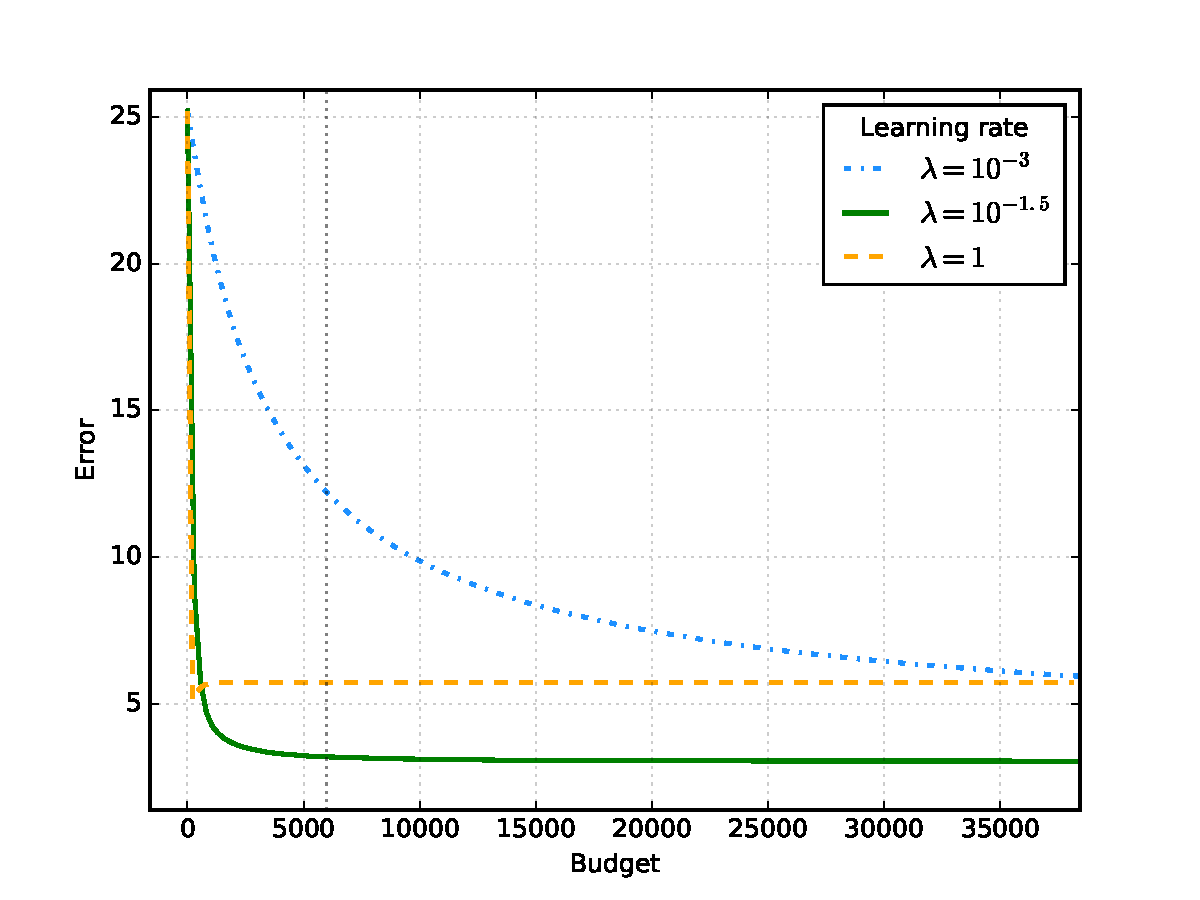
\includegraphics[width=\columnwidth]{friedman1_lr}}
\caption{Friedman1: Testing set mean square error with respect to the budget 
($CW=\infty$, m=$\sqrt{10}$, $T=1000$, budget=$59900$ ($10\%$)).}
\label{fig:learningRate}
\end{center}
\vskip -0.2in
\end{figure} 

\subsection{Influence of the hyper-parameters}

\paragraph{Learning rate}
Figure \ref{fig:learningRate} depicts a typical evolution of the error with the 
budget in the case of Friedman1 (the budget of $59900$ corresponds to $10\%$). 
A unit learning rate will usually decrease the test set error rapidly 
but will then either saturates or overfits. Too small a learning rate ({\it 
e.g.} $10^{-3}$) will prevent the model from reaching its minimum in the 
alloted budget.  The learning rate also influences the forest's shape, provided 
the candidate window size is large enough. On Figure \ref{fig:LRShape}, we can 
see that, for the smallest learning rate, the $80\%$ of the smallest trees 
account for $43\%$ of nodes. At that stage, only $17\%$ and $13\%$ of the nodes 
are covered for the average and biggest learning rates, respectively.


\begin{figure}[ht]
\begin{center}
\centerline{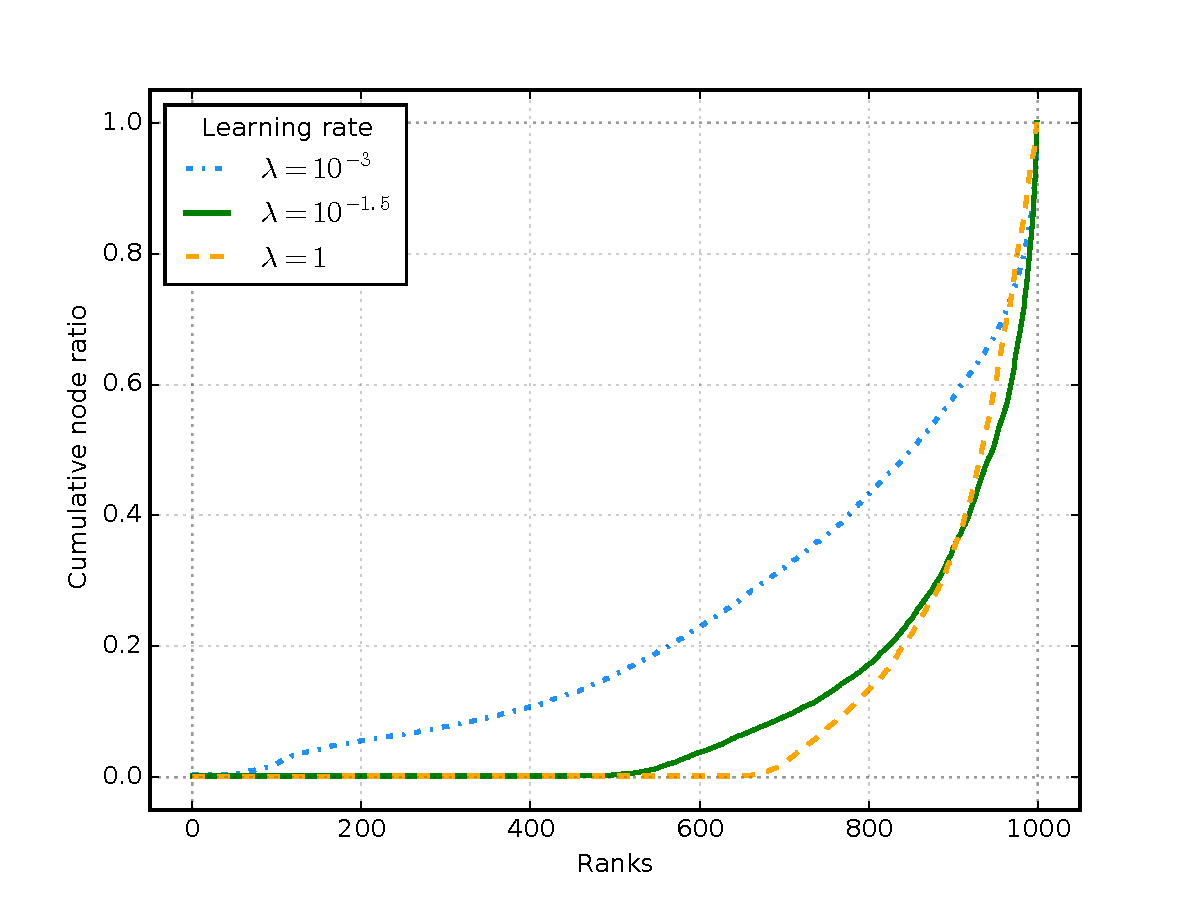
\includegraphics[width=\columnwidth]{friedman1_cumul}}
\caption{Friedman1: node distribution across tree ($CW=\infty$, 
m=$\sqrt{10}$, $T=1000$, budget=$59900$ ($10\%$).}
\label{fig:LRShape}
\end{center}
\vskip -0.2in
\end{figure} 

\paragraph{Number of features}

\paragraph{Candidate window size}
CW=1, CW=10, CW=inf
Performance + time

\paragraph{Number of trees}
With CW=inf, With CW=1

\subsection{Comparison with Boosting}

%\subsection{Comparison with post-pruning}













\appendix
\section{Equivalence of GIF and the underlying tree}\label{app:Equiv}
In the case of a single tree and a unit learning rate, both the square loss in 
regression and the multiexponential loss in classification produce the same 
prediction as the underlying tree. 
This is due to the fact that, when examining the weight to give to node $j$ at 
time $t$, the prediction of time $t-1$ relates to the parent $\pi_j$ of $j$. It 
is thus independent of $t$ and is also the same for all instance reaching that 
node. Consequently, we will adopt the following slight change in notation:

\begin{align}
\hat{y}_j = \hat{y}_{(\pi_j)} + w_j
\end{align}

Meaning that the prediction associated to any object reaching node $j$ is the 
weight of $j$ plus the prediction associated to its parent $\pi_j$. With 
$\hat{y}_{(\pi_1)} = 0$, the prediction of the root's pseudo-parent.

\subsection{Regression}
In regression, the tree prediction $Tr_j$ of any leaf $j$ is the average of the 
learning set's outputs reaching that node: $Tr_j = \frac{1}{|Z_j|}\sum_{i \in 
Z_j} y_i$. We need to show that the GIF prediction is:

\begin{align}\label{eq:EquivL2Cond}
\hat{y}_{j} = \frac{1}{|Z_j|}\sum_{i \in Z_j} y_i
\end{align}


The prediction of node $j$ is

\begin{align}\label{eq:EquivL2Solution}
\hat{y}_j &= \hat{y}_{\pi_j} + w_j \\
&= \hat{y}_{\pi_j} +  \frac{1}{|Z_j|} \sum_{i \in Z_j} \left(y_i - 
\hat{y}_{\pi_j}\right) \\
&= \hat{y}_{\pi_j} + \frac{1}{|Z_j|} \sum_{i \in Z_j} \left( y_i \right) - 
\hat{y}_{\pi_j} \\
&= \frac{1}{|Z_j|} \sum_{i \in Z_j}  y_i 
\end{align}
The first step is how the additive model is built. The second is the optimal 
weight value of node $j$ derived in Equation \ref{eq:L2Solution}, the third 
step is due to the fact that the prediction at $\pi_j$ is constant since there 
is only one tree.

\subsection{Classification}
In order to have the same prediction as the underlying tree, we must 
demonstrate that the probability of being in class $l$ associated to node $j$ 
will be $\frac{Z_j^{(l)}}{|Z_j|}$.
Under the zero-sum constraint, we have

\begin{align} 
\exp \left(  \frac{1}{K-1} w_j^{(l)}\right) &= \frac{1}{c_j} 
\alpha_{\pi_i}^{(l)} \\
&=  \frac{1}{c_j} \sum_{i \in Z_j^{(l)}} \exp \left(-\frac{1}{K-1} 
\hat{y}_{\pi_i}^{(l)}\right)\\
&= |Z_j^{(l)}| \exp \left(-\frac{1}{K-1} \hat{y}_j^{(l)}\right) \\
\exp \left(\frac{1}{K-1} \hat{y}_j^{(l)} \right) &= \exp \left(\frac{1}{K-1} 
\hat{y}_{\pi_j}^{(l)} \right) \exp \left(\frac{1}{K-1} w_j^{(l)}\right) \\
&= \frac{1}{c_j} |Z_j^{(l)}| \\
P_j(l) &= \frac{\exp \left(\frac{1}{K-1} \hat{y}_j^{(l)}
\right)}{\sum_{k=1}^K\exp \left(\frac{1}{K-1} \hat{y}_j^{(k)} \right)} = 
\frac{|Z_j^{(l)}|}{|Z_j|}
\end{align}

where $c_j = \left(\prod_{k=1}^K \alpha_j^{(k)}\right)^{\frac{1}{K}}$ is a 
constant. The first equality is a consequence of the value of $w_j^{(l)}$ 
(Equation \ref{eq:MEsolution}). The second is a due to the definition of 
$\alpha_j^{(l)}$ (Equation \ref{eq:MEClsErrZS}). The third is a consequence of 
having a single tree: the prediction of the parent is the same for all 
instances.





Notice that, in both regression and classification, the equivalence also holds 
for an internal node: the prediction is the one the tree would have yielded if 
that node had been a leaf.


\bibliography{gif}
\bibliographystyle{icml2016}

\end{document} 

